\subsection{MVC}

\enquote{Model-View-Controller}, herefter kaldt MVC, er et designmønster, der bruges til at strukturere software med en brugergrænseflade \cite{mvcLecture}. Mønsteret opdeler en given software applikation i tre sammenhængende dele. Det centrale komponent, \enquote{Model}, som indeholder data og modellerer problemområdet. Et ydre komponent, \enquote{View}, der afvikler den visuelle repræsentation af information til brugeren. Den tredje del, \enquote{Controlleren}, som implementerer systemets funktionaliteter. Fordelen ved MVC er at programmet struktureres på en måde, så programmets enkelte dele har en lav kobling. En lav kobling gør det nemmere at udskifte dele af et program, og derved bliver programmet nemmere at vedligeholde. For eksempel kan hele det grafiske framework udskiftes, ved blot at skifte det ydre \enquote{View} komponent ud. \Cref{fig:mvc} viser den tydelige strukturelle forskel på \enquote{Model}, \enquote{View} og \enquote{Controller} komponenterne.

\begin{figure}
  \centering
  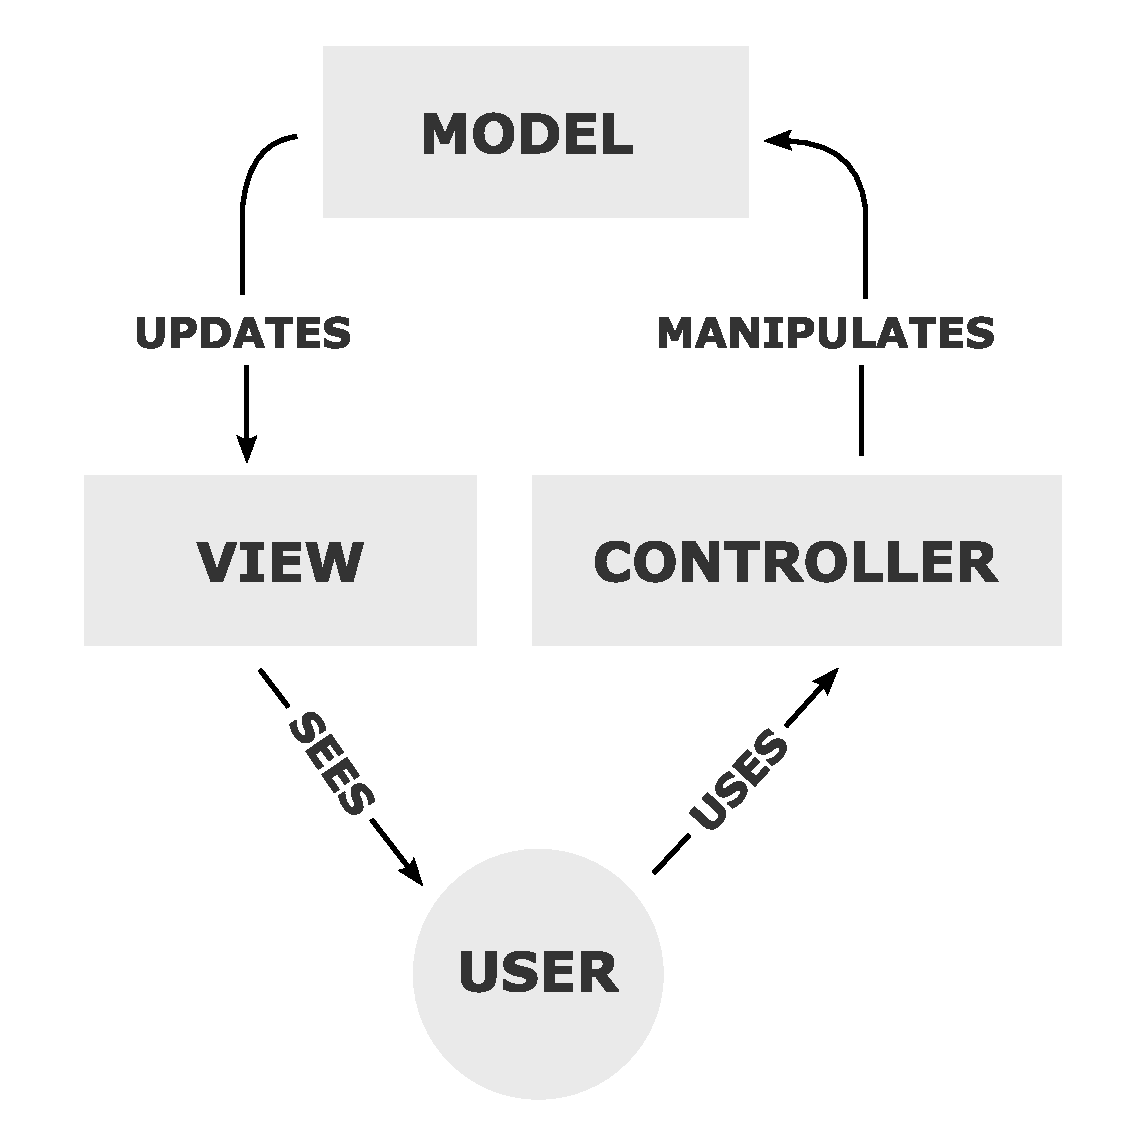
\includegraphics[width=0.75\textwidth]{mvc.pdf}
  \caption{Grundidéen omkring MVC. Fra \url{http://en.wikipedia.org/wiki/Model-view-controller} } \label{fig:mvc}
\end{figure}
